%!TEX encoding=UTF-8 Unicode
\section{Expriments}
\label{sec:expe}
In this section, we show how to analyse and optimize NUMA memory behaviour using
\TABARNAC through two benchmarks. Finally we discuss our tool overhead.
\subsection{Setup}
\label{sec:expe-setup}
machines used, becnhmarks, tools, mechanism used \ldots

\DB{fill the tabular}
\begin{table}
    \centering
    \resizebox{\linewidth}{!}
    {
        \begin{tabular}{l|c|c|l|c|c|l}
            Machine & \#Numa nodes & \#Core & CPU & Cache (Mib) & Mem (GiB) & OS\\
            \hline
            Turing & 4 & 64 & ?? & ?? & ?? &  ubuntu ??\\
            \hline
            Naskapi & ?? &?? &?? &?? & ?? &debian ??\\
        \end{tabular}
    }
    \caption{Experimental machine description}
    \label{tab:machines}
\end{table}

\subsection{Analysis}
\label{sec:expe-analysis}

\subsubsection{IS}
The first benchmark we studied is \emph{IS} from the  NAS Parallel benchmarks OpenMp
\cite{Feng04Unstructured}. This applications computes a bucket sort using
mainly three arrays.

\begin{figure}[htb]
    \centering

    \subfigure[\texttt{key\_buff2}]{
        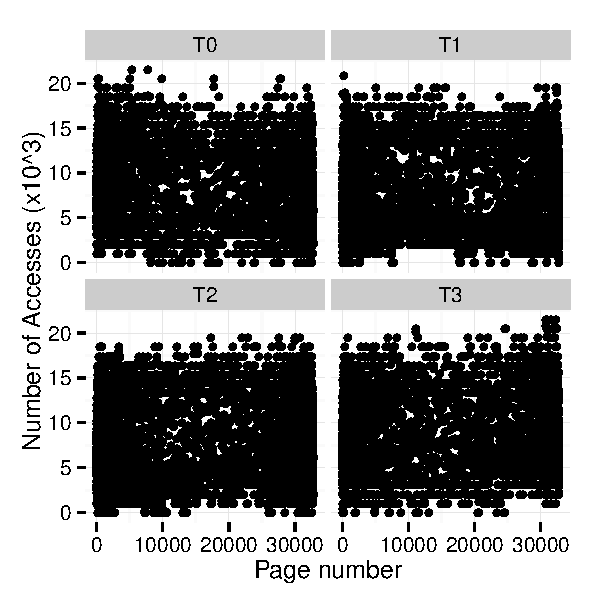
\includegraphics[width=.45\linewidth] {is_w_kb2_orig}
        \label{fig:is-behaviour-orig-kb2}
    }
    \subfigure[\texttt{key\_array}]{
        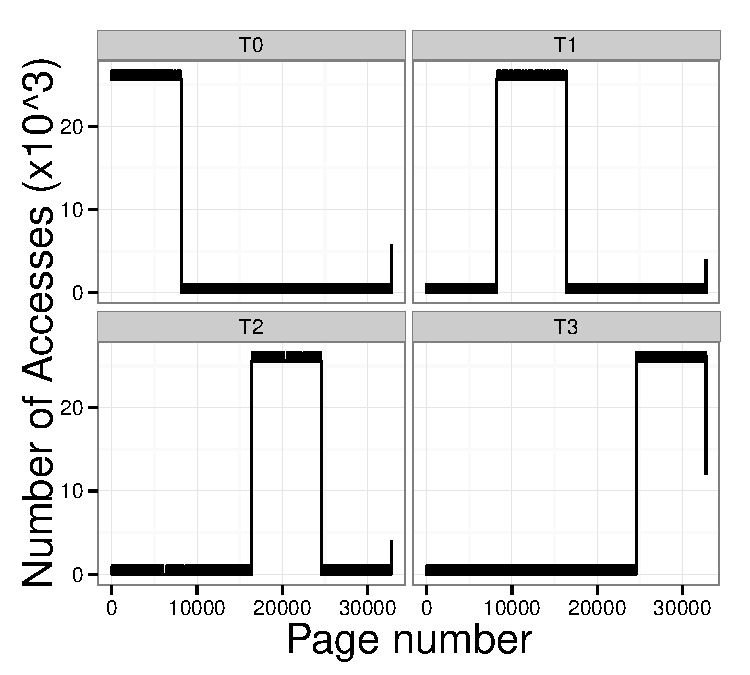
\includegraphics[width=.45\linewidth] {is_w_kba_orig}
        \label{fig:is-behaviour-orig-kba}
    }

    \subfigure[\texttt{key\_buff1}]{
        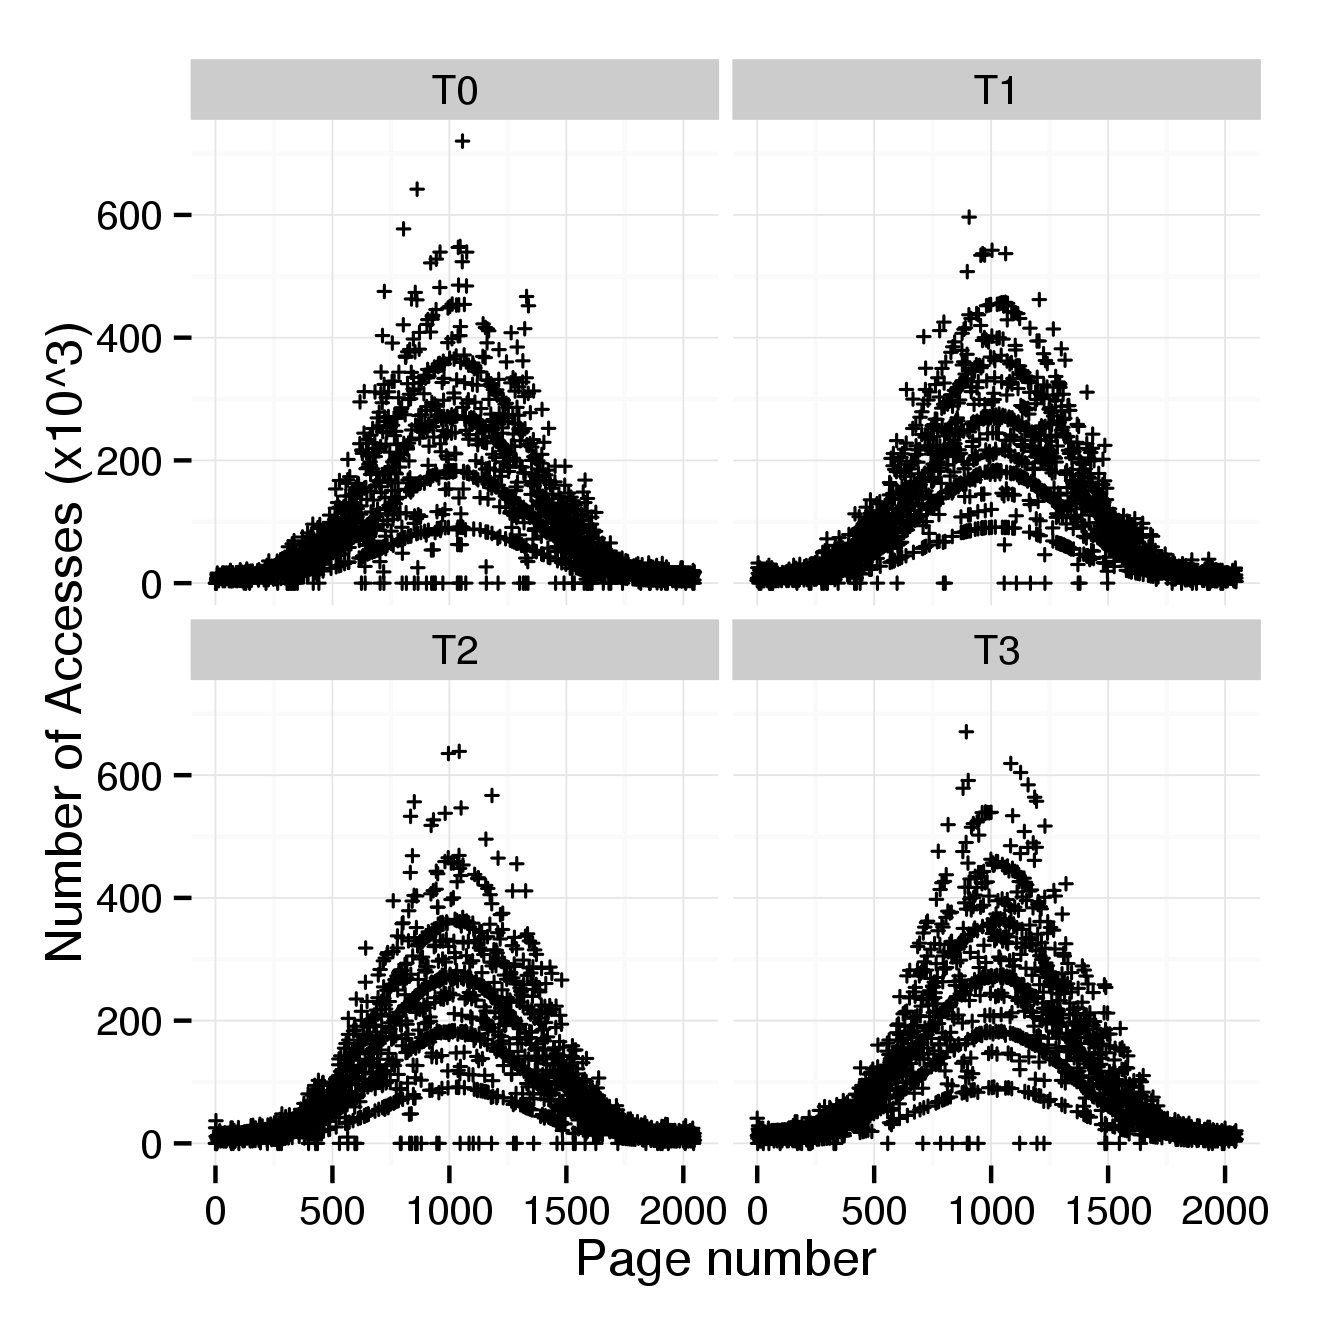
\includegraphics[width=.45\linewidth] {is_w_kb1_orig}
        \label{fig:is-behaviour-orig-kb1}
    }
    \caption{Original memory access distribution for the main structure of
        \emph{IS} with $4$ threads.}
    \label{fig:is-behaviour-orig}
\end{figure}

Figure \ref{fig:is-behaviour-orig} shows the access distributions for the
three main structures of \emph{IS} class W with $4$ threads. We can see that
each of these structure have a different access pattern: \texttt{key\_array}
(fig \ref{fig:is-behaviour-orig-kba}) access distribution shows that every
threads works on a different part of the structures which allows automated
tools to do efficient data/thread mapping on it. However \texttt{key\_buff2}
(fig \ref{fig:is-behaviour-orig-kb2}) is completely shared by every threads,
but the most interesting access distribution is the one of \texttt{key\_buff1}
(fig \ref{fig:is-behaviour-orig-kb1}). Indeed the access repartition seems to
follow a nice Gaussian, which means a few pages are more used than all the
others. Finding a good numa balance with such a distribution is difficult and
almost impossible for automated tools.


\lstinputlisting[caption=\emph{IS} code responsible for the
Guassain distribution of access, label=lst:is]{code/is.c}

Using this knowledge, we can look at \emph{IS} code and identify the source of the
Gaussian pattern, indeed all the access to \texttt{key\_buff1} are linear
excepts the one shown in listing \ref{lst:is}\footnote{
    The code have been slightly modified to make it more readable. In the
    original version the arrays \texttt{key\_buff1} (resp \texttt{key\_buff2})
    are accessed via a generic pointer called \texttt{key\_buff\_ptr} (resp
    \texttt{key\_buff\_ptr2}). More over some comments have been removed as
    they are not necessary here.
}  line \ref{lst:is-gaus}-\ref{lst:is-gaus-end} which depends on the values of
\texttt{key\_buff2}. The comments above the OpenMp loop explains that the
cyclic distribution will result in an unbalanced work distribution. Still we can easily design a cyclic
distribution aware of the Gaussian pattern which provides both a good
distribution of access among the thread and a strong locality. The idea is to
split the loop in two half and give one part of each half to each threads in a
round robin way. We can do that only by modifying line \ref{lst:is-cyclic} as
shown in listing \ref{lst:is-modif}.
\begin{lstlisting}[caption=One line optimization for \emph{IS}, label=lst:is-modif]
#pragma omp for schedule(static,NUM_BUCKETS/(2*omp_get_max_threads()))
\end{lstlisting}

\begin{figure}[htb]
    \centering

    \subfigure[\texttt{key\_buff2}]{
        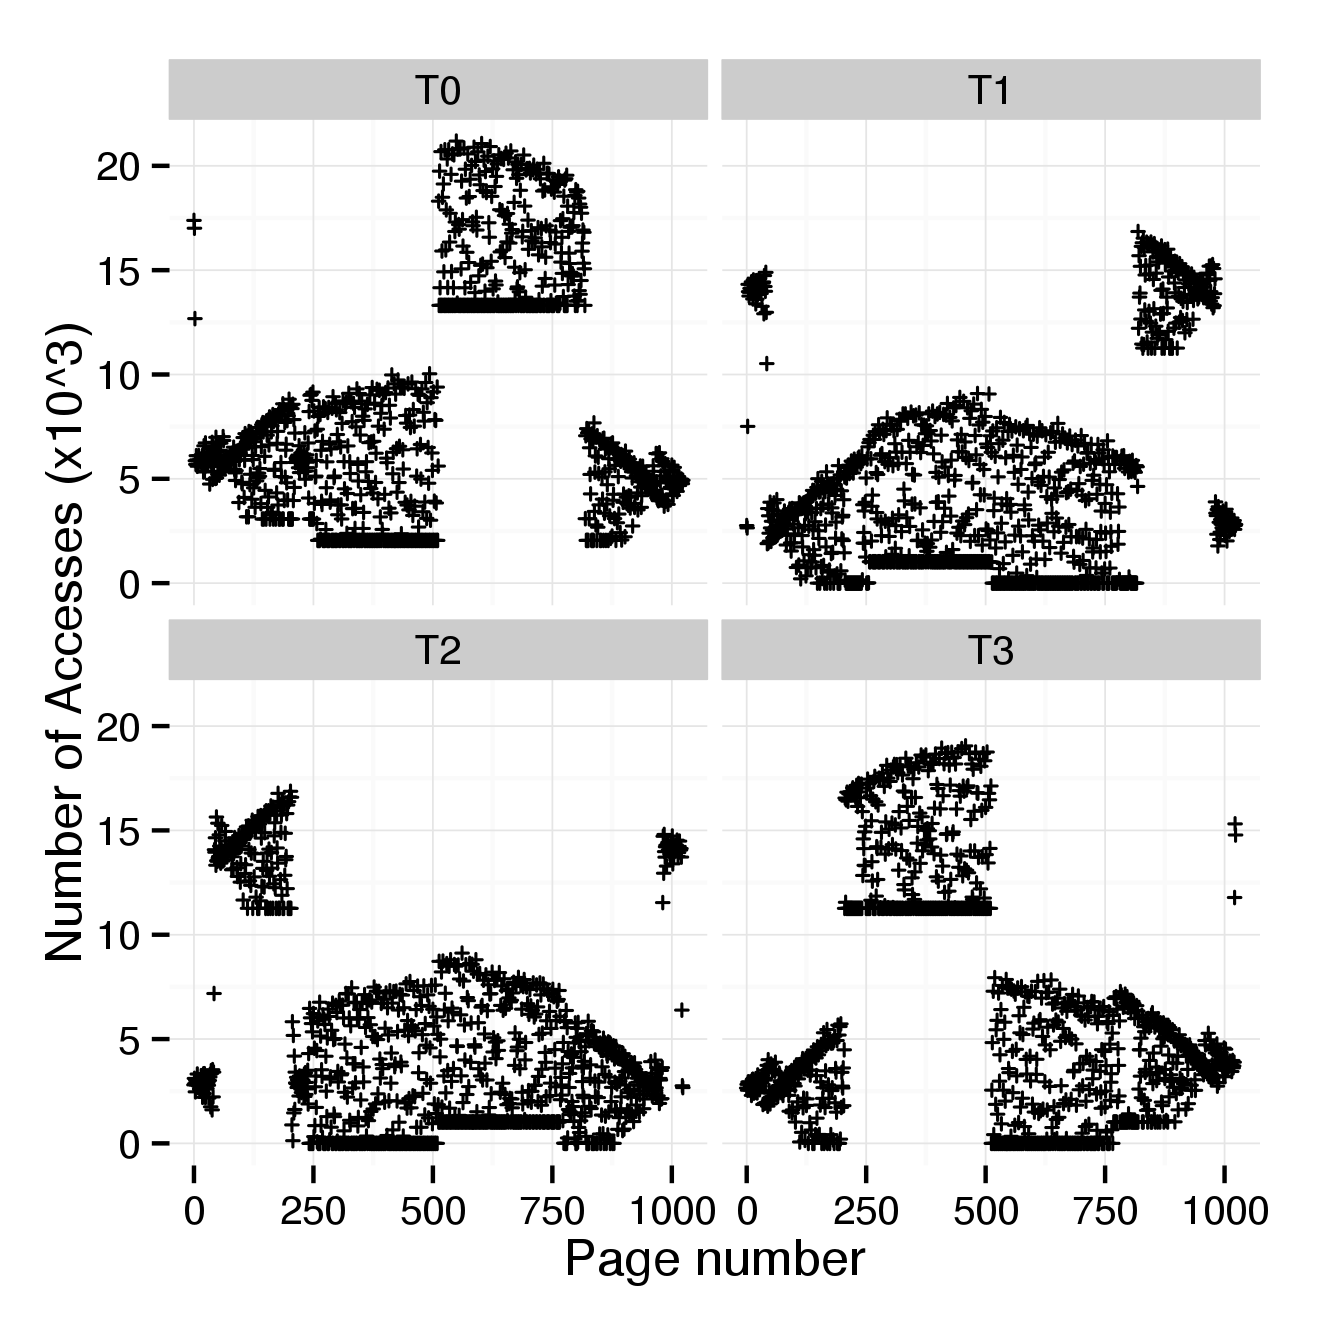
\includegraphics[width=.45\linewidth] {is_w_kb2_modif}
        \label{fig:is-behaviour-modif-kb2}
    }
    \subfigure[\texttt{key\_array}]{
        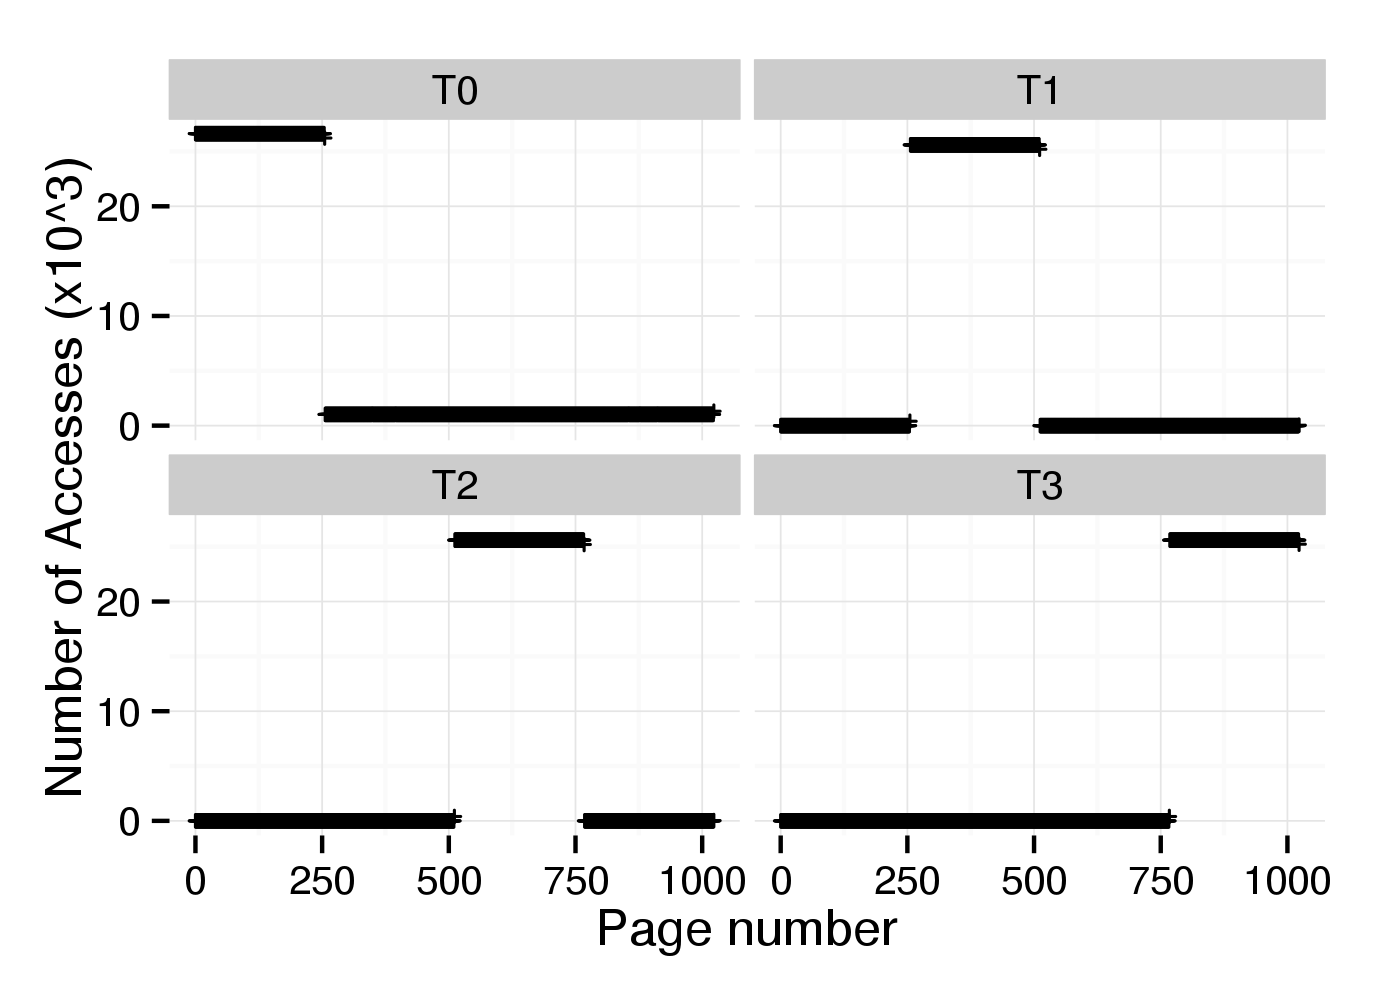
\includegraphics[width=.45\linewidth] {is_w_kba_modif}
        \label{fig:is-behaviour-modif-kba}
    }

    \subfigure[\texttt{key\_buff1}]{
        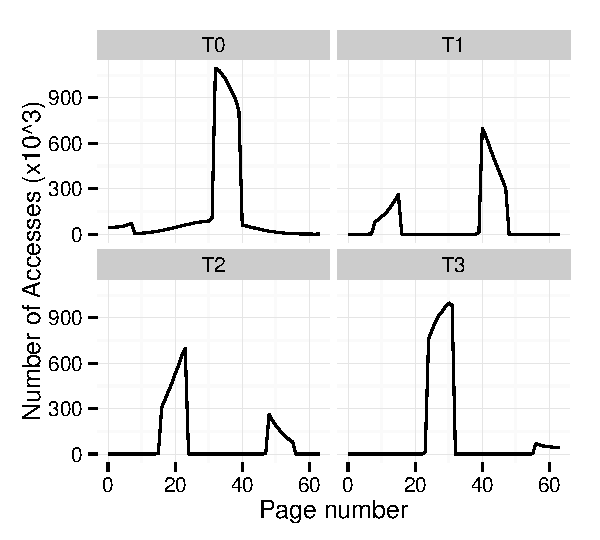
\includegraphics[width=.45\linewidth] {is_w_kb1_modif}
        \label{fig:is-behaviour-modif-kb1}
    }
    \caption{Memory access distribution for the main structure of
        \emph{IS} with $4$ threads after our modifications.}
    \label{fig:is-behaviour-modif}
\end{figure}

With this extremely simple code modification we obtain the access distribution
shown in figure \ref{fig:is-behaviour-modif}. We can see that not only it fixed
the distribution of \texttt{key\_buff1} but \texttt{key\_buff2} have also a
better exclusivity now.
\DB{developp: gaussian is smoother blalbla}

We then compare the execution time of the three distribution: \emph{Dynamic},
\emph{Cyclic} with a step of $1$ and \emph{Tabarnac}: cyclic with the
distribution proposed bot with and without numa balancing enabled.


\begin{figure}[htpb]
    \centering
    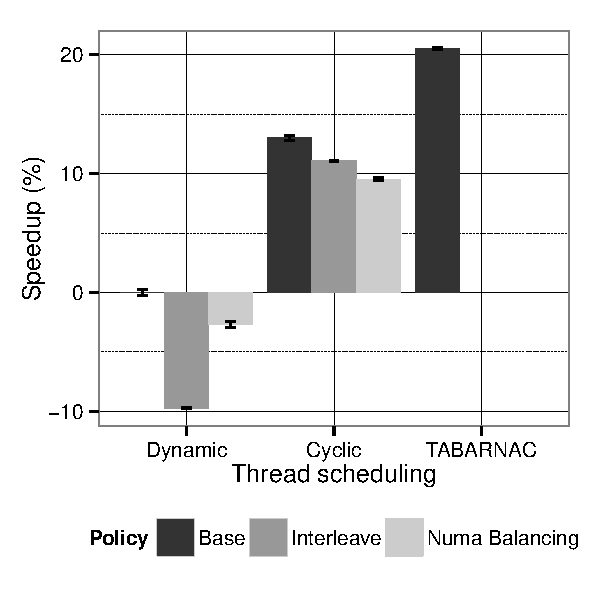
\includegraphics[width=.9\linewidth]{is_exectime.pdf}
    \caption{Execution time of \emph{IS} in class D under the different
configurations.}
\label{fig:is-res}
\end{figure}

Figure\ref{fig:is-res} show the execution time \emph{IS} in class D for each
configuration. We can see that our optimization provides the best results for
both configuration.  Moreover \emph{numa balancing} is not efficient for
\emph{IS}. This behaviour seems to come from the fact that the first touch is
almost always done by the thread actually using the data, therefore the gain
provided by \emph{numa balancng} is not enough to compensate the runtime
overhead.
\DB{Evaluate the parallel time / seq time to discuss the gain}

\subsubsection{Stream Cluster}
same methodo as above

